\documentclass{standalone}
\usepackage{tkz-fct}
\usepackage{tkz-euclide}
\usepackage{color}
\usepackage{amsmath}
\renewcommand*\familydefault{\sfdefault}
\usepackage{sansmath}
\sansmath
\definecolor{gray75}{gray}{0.75}
\begin{document}
 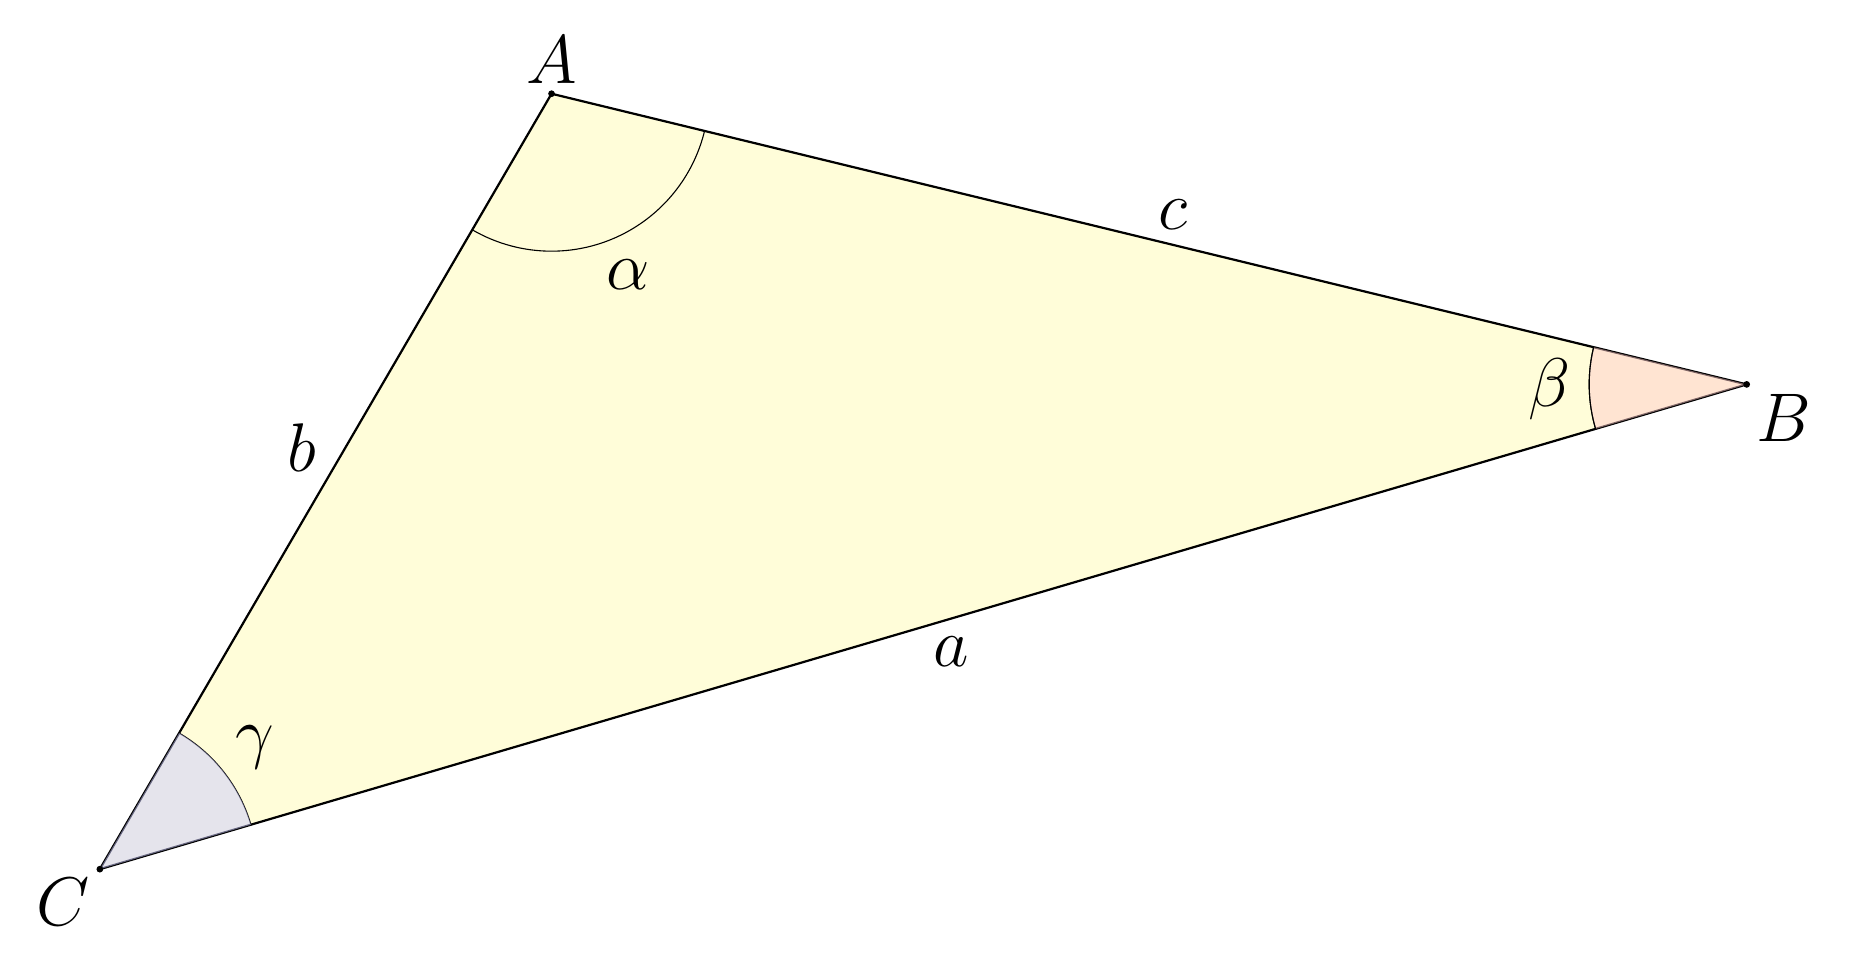
\begin{tikzpicture}[scale=2]
   
    \tkzDefPoint["\Huge $C$" below left](-2,0){C}
    \tkzDefPoint["\Huge $B$" below right](20:9){B}
    \tkzDefPoint["\Huge $A$" above](80:5){A}
    \tkzDefPointsBy[projection=onto B--C](A){a}
    \tkzDrawPolygon[thick,fill=yellow!15](A,B,C)
    \tkzMarkAngle(B,C,A)
    \tkzMarkAngle(C,A,B)
    \tkzMarkAngle(A,B,C)
    \tkzFillAngle[fill=blue!20, opacity=0.5](B,C,A)
    \tkzFillAngle[fill=red!20, opacity=0.5](A,B,C)
    \tkzLabelAngle[pos=1.25](A,B,C){\Huge $\beta$}
    \tkzLabelAngle[pos=1.25](B,C,A){\Huge $\gamma$}
    \tkzLabelAngle[pos=1.25](C,A,B){\Huge $\alpha$}
    \tkzLabelSegment[below right](C,B){\Huge $a$}
    \tkzLabelSegment[above left](A,C){\Huge $b$}
    \tkzLabelSegment[above right](A,B){\Huge$c$}
    \tkzMarkAngle(A,B,C)
    \tkzDrawPoints(A,B,C)

\end{tikzpicture}
\end{document}
